\documentclass[a4paper, twoside, 12pt]{article}
\usepackage{outline}
\usepackage{pmgraph}
\usepackage[normalem]{ulem}
\usepackage{amsmath}
\usepackage{listings}
\usepackage{lipsum}
\usepackage{layout}
\usepackage{indentfirst}
\usepackage[brazilian]{babel}
\usepackage{float}
\usepackage[utf8]{inputenc}
\usepackage[T1]{fontenc}
\usepackage{lingmacros}
\usepackage{tree-dvips}
\usepackage{multirow}
\usepackage{caption}
\usepackage{subcaption}
\usepackage{titlesec}
\usepackage{chngcntr}
\usepackage{indentfirst}
\usepackage{hyperref}

% Images
\usepackage{graphicx}
\usepackage{txfonts}
\usepackage{graphics}


% \setcounter{secnumdepth}{5}

\titleformat{\paragraph}
{\normalfont\normalsize\bfseries}{\theparagraph}{1em}{}
\titlespacing*{\paragraph}
{0pt}{3.25ex plus 1ex minus .2ex}{1.5ex plus .2ex}

\numberwithin{equation}{section}

\title{\textbf{CC298 - Projetos}}
\author{Leonardo Motta Maia de Oliveira Carvalho}
\date{\oldstylenums{00}/\oldstylenums{00}/\oldstylenums{00}}

%--------------------Make usable space all of page
\setlength{\oddsidemargin}{0in}
\setlength{\evensidemargin}{0in}
\setlength{\topmargin}{0in}
\setlength{\headsep}{-.25in}
\setlength{\textwidth}{6.5in}
\setlength{\textheight}{8.5in}
\counterwithin{paragraph}{subsubsection}

%--------------------Indention
\setlength{\parindent}{1cm}

\begin{document}
\bibliographystyle{plain}
%--------------------Title Page
\maketitle
\tableofcontents
 
%--------------------Begin sections
\begin{abstract}
    \textit{Este relatório tem  como objetivo apresentar os estudos feitos ao
    longo da disciplina CC298 ministrada ao longo do ano de 2018. Os projetos
    propostos na disciplina concentravam-se no problema do bocal convergente
    divergente. Para resolver o problema do bocal, a formulação de Euler foi
    usada. Para discretizar as equações, uma malha estruturada de bloco único
    foi usada em conjunto com uma transformação de coordenadas que
    possibilitava a representação de geometrias curvilíneas. Alguns dos
    esquemas propostos foram implementados e testados. O objetivo desse
    relatório é documentar os avanços feitos no estudo dos métodos de marcha no
    tempo implicitos e nos esquemas de discretização espacial.}
\end{abstract}

\section{Bocal Convergente-Divergente}

Descrever o bocal.

\section{Formulação Teórica}

\subsection{Equações de Euler}
Equações de Euler.
\begin{equation}
\frac{\partial U}{\partial t}+\frac{\partial F(U)}{\partial x}+\frac{\partial G(U)}{\partial y}=0.
\end{equation}

\subsection{Transformação de Coordenadas}
Falar sobre a transformação de coordenadas.

\section{Formulação Numérica}

\subsection{Esquema Centrado}

\subsubsection{Operadores de Dissipação Artificial}

\subsection{Esquema de Beam-Warming}

\subsection{Esquema de Steger-Warming}


\section{Resultados e discussões}
Falar sobre os resultados.
        \begin{figure}[htb]
            \centering
            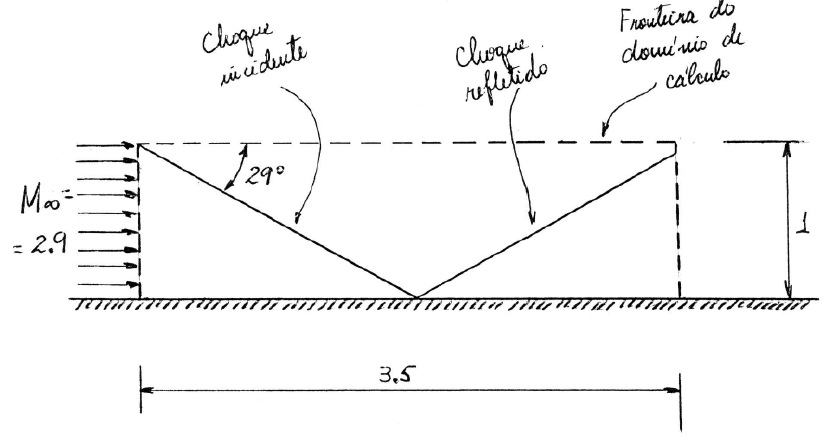
\includegraphics[width=.7\linewidth,height=50mm]{pics/shock.png}
            \caption{Esquematização do problema resolvido \cite{AZEVEDO}}
            \vspace*{-5pt}
        \end{figure}

    \subsection{Malhas usadas}
        \begin{figure}[H]

        \begin{subfigure}{.5\textwidth}
        \centering
        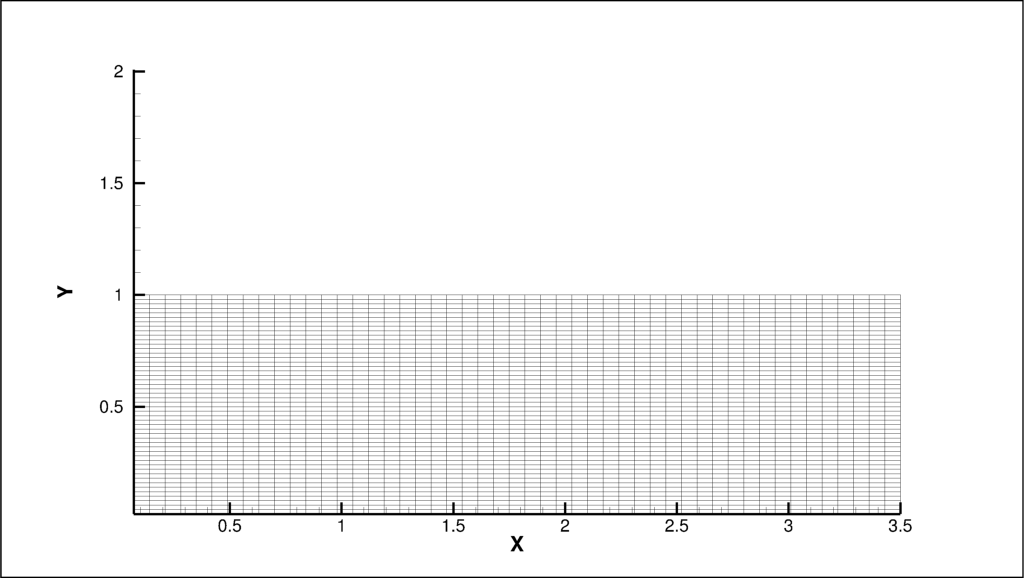
\includegraphics[width=.9\linewidth]{pics/mesh_5050.png}
        \caption{Malha com $50x50$ pontos}
        \label{fig:sfig1}
        \end{subfigure}%
        \begin{subfigure}{.5\textwidth}
        \centering
        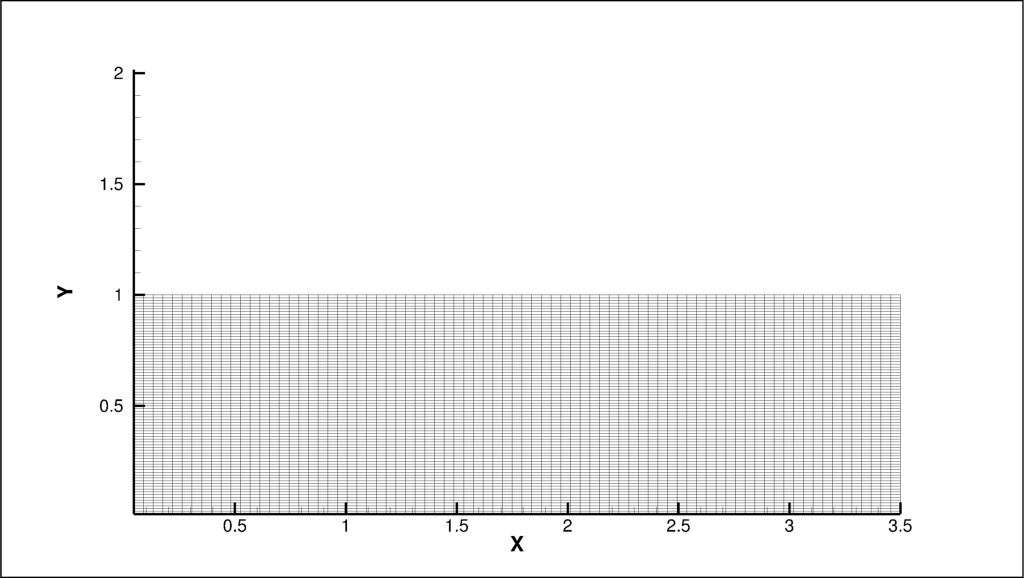
\includegraphics[width=.9\linewidth]{pics/mesh_8080.png}
        \caption{Malha com $80x80$ pontos}
        \label{fig:sfig2}
        \end{subfigure}
        \\
        \begin{subfigure}{.5\textwidth}
        \centering
        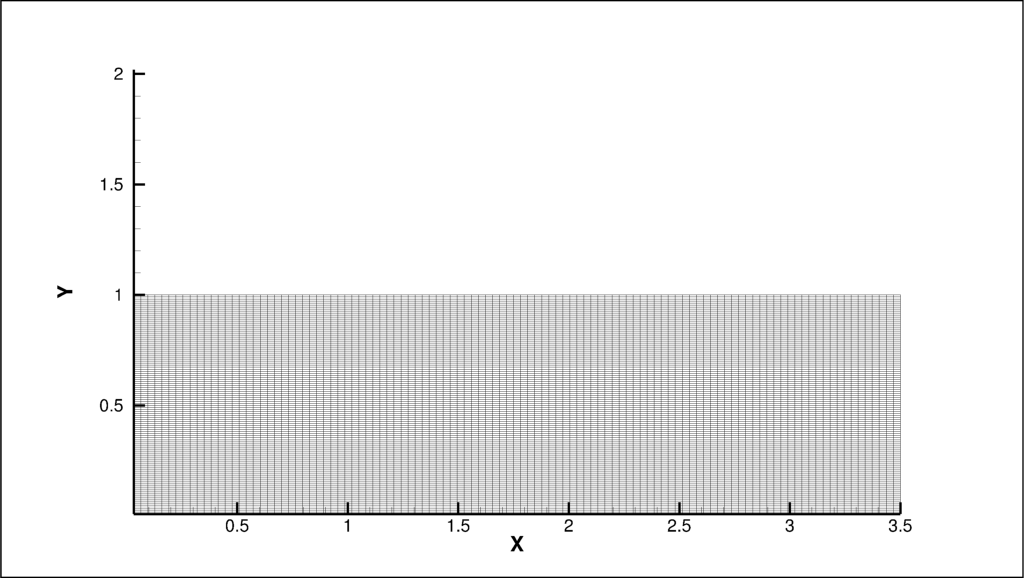
\includegraphics[width=.9\linewidth]{pics/mesh_110110.png}
        \caption{Malha com $110x110$ pontos}
        \label{fig:sfig1}
        \end{subfigure}%
        \begin{subfigure}{.5\textwidth}
        \centering
        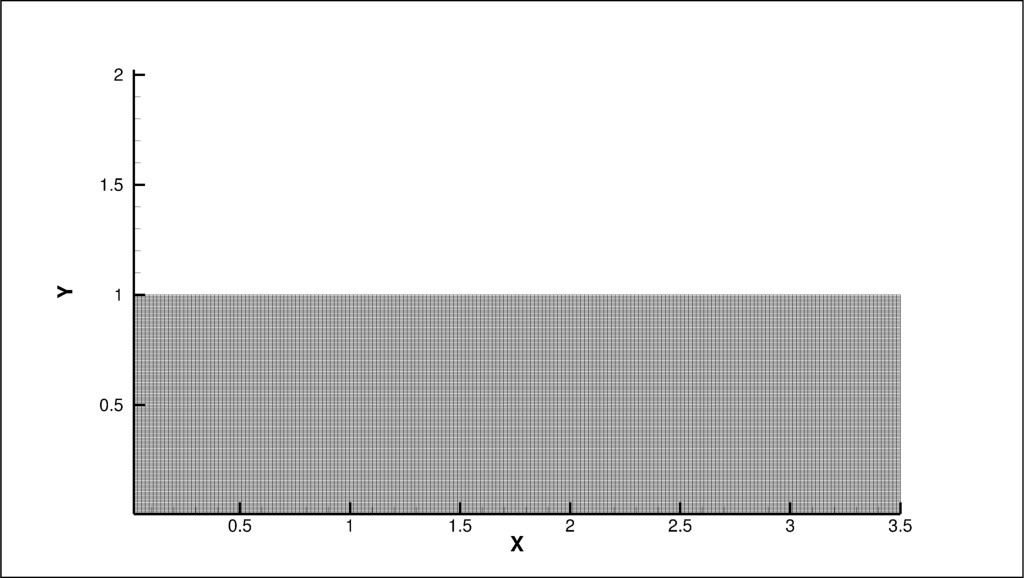
\includegraphics[width=.9\linewidth]{pics/mesh_200200.png}
        \caption{Malha com $200x200$ pontos}
        \label{fig:sfig2}
        \end{subfigure}

        \caption{Malhas usadas durante os cálculos.}
        \label{fig:fig}
        \vspace*{-5pt}
        \end{figure}

    \subsection{Desempenho computacional e numérico}
Nesta seção serão apresentados os resultados referentes ao desempenho numérico e às comparações com a solução analítica.

\subsection{Conclusões}

Bostejar as conclusões.

\bibliography{refs.bib}

\end{document}

